\documentclass[fleqn]{article}
\usepackage[utf8]{inputenc}
\usepackage{amsmath}
\usepackage{lmodern} % for bold teletype font
\usepackage{listings}
\usepackage[export]{adjustbox}
\usepackage{subcaption}
\usepackage{graphicx}
\usepackage{xcolor}   % for \textcolor
\usepackage{float}

\lstset{
  basicstyle=\ttfamily,
  columns=fullflexible,
  frame=single,
  breaklines=true,
  postbreak=\mbox{\textcolor{red}{$\hookrightarrow$}\space},
}


\title{Static Resource Allocation}
\author{Mark Towers}
\date{June 2019}

\begin{document}
\maketitle

\section{Problem Statement}\label{sec:problem-statement}
In prior research into resource pricing for resource allocation within cloud computing, job's considered have had fixed resource requirements that server's must fulfill.
However in this research we consider job's that have requirements that must be fulfill with a deadline so that the resource allocation must allow the deadline consider to be true.
We have then developed a greedy algorithm to solve the problem to maximise the social welfare where the total utility is known of ecah jobs.
However in real life then server's that run the job would want to be payed to run a job so we have developed new auction. \\
In the new section, we will describe the problem case and how we generated a model. \\

\section{Problem Case}\label{sec:problem-case}
\subsection{Variable}\label{subsec:variable}
There are J jobs, indexed with $ j = 1,\dots,J $ and I servers, indexed with $ i = 1,\dots,I $.
\begin{itemize}
    \item $ x_{i,j} \in \{0, 1\}$ indicates whether the job $j$ was done on server $i$
    The rate at which the server resources are used for each job
    \item $ s_{i,j} $ the rate of the program loaded (MB/s)
    \item $ w_{i,j} $ the rate of computation (TFlop/s)
    \item $ r_{i,j} $ the rate of sending the results data (MB/s)
\end{itemize}

\subsection{Constants}\label{subsec:constants}
Server - i
\begin{itemize}
    \item Maximum storage - $ S_i $ (MB)
    \item Maximum computation capacity - $ W_i $ (TFlop/s)
    \item Maximum communication bandwidth - $ R_i $ (MB/s)
\end{itemize}
Job - j
\begin{itemize}
    \item Required storage - $ s_j $ (MB)
    \item Required computation capacity - $ w_j $ (TFlop)
    \item Required data for results - $ r_j $ (MB)
    \item Utility - $ U_j $ (\$)
    \item Deadline - $ D_j $ (s)
\end{itemize}

\subsection{Optimisation}\label{subsec:optimisation}
\begin{align}
    max \sum_{j=1}^{J} U_j x_{i,j} && \forall i = 1,\dots,I
\end{align}
s.t.

\subsection{Constraints}\label{subsec:constraints}
Job to server allocation
\begin{align}
    \sum_{i=1}^I x_{i,j} \leq 1 && \forall j = 1,\dots,J \\
    x_{i,j} \in \{0, 1\} && \forall i = 1,\dots,I; j = 1,\dots,J
\end{align}

%% Server resources checking
Server resource available
\begin{align}
    \sum_{j=1}^J s_j x_{i,j} \leq S_i && \forall i = 1,\dots,I
\end{align}
\begin{align}
    \sum_{j=1}^J w_{i,j} x_{i,j} \leq W_i && \forall i = 1,\dots,I
\end{align}
\begin{align}
    \sum_{j=1}^J (r_{i,j} + s_{i,j}) x_{i,j} \leq R_i && \forall i = 1,\dots,I
\end{align}

%% Within deadline
Process completed within deadline
\begin{align}
    \frac{S_j}{s_{i,j}} + \frac{W_j}{w_{i,j}} + \frac{R_j}{r_{ij}} \leq D_j && \forall i = 1,\dots,I; j = 1,\dots,J
\end{align}

Resource usage
\begin{align}
    0 \le s_{i,j} && \forall i = 1,\dots,I; j = 1,\dots,J
\end{align}
\begin{align}
    0 \le w_{i,j} && \forall i = 1,\dots,I; j = 1,\dots,J
\end{align}
\begin{align}
    0 \le r_{i,j} && \forall i = 1,\dots,I; j = 1,\dots,J
\end{align}

\subsection{Problem Case Explaination}\label{subsec:problem-case-explaination}
\begin{itemize}
    \item Equation 1 is the objective function that maximises the sum of the job utility for jobs completed.
    \item Equation 2 and 3 enforce that a job is only done on a single server.
    \item Equations, 4 to 6, ensures that the server resource used are within the maximum resources available.
    \item Equation 7 enforces that the job will be completed within the deadline on only the servers that is a job runs on.
    \item Equations, 8 to 10, ensures that resource speeds are within a valid range of greater than 0
\end{itemize}

\subsection{Example cases}\label{subsec:example-cases}
\begin{figure}[H]
    \begin{subfigure}{0.5\textwidth}
        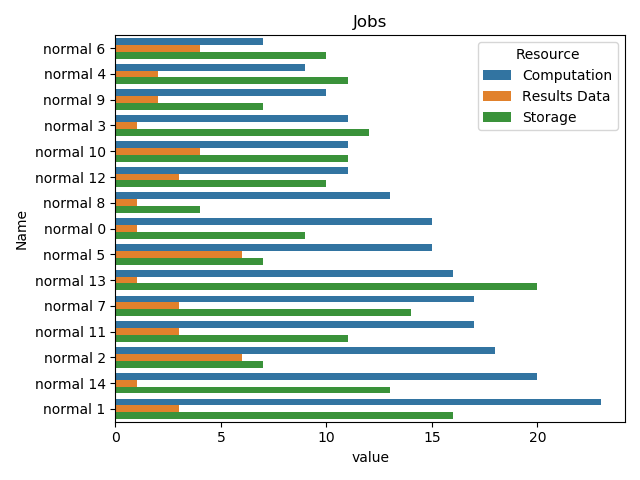
\includegraphics[width=1\linewidth, height=5cm]{../results/jobs.png}
        \caption{Example jobs}
    \end{subfigure}
    \begin{subfigure}{0.5\textwidth}
        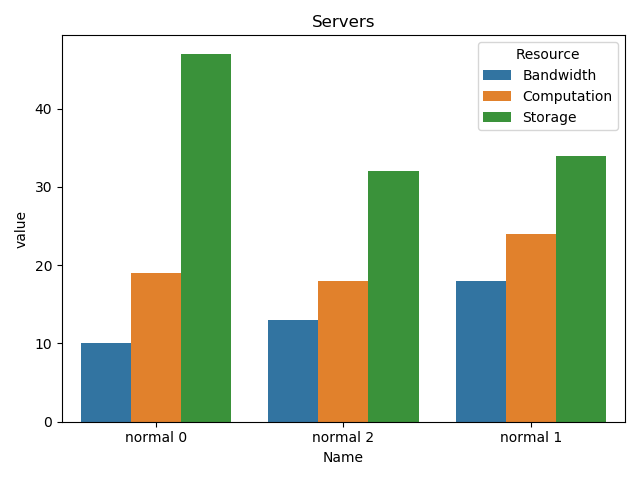
\includegraphics[width=1\linewidth, height=5cm]{../results/servers.png}
        \caption{Example Servers}
    \end{subfigure}

    \caption{Example jobs and servers}
\end{figure}

\begin{figure}[H]
    \centering
    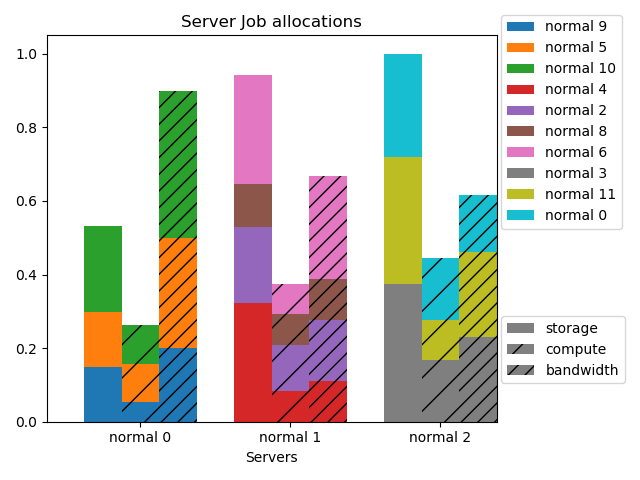
\includegraphics[width=1\textwidth]{../results/greedy_allocation.png}
    \caption{Server and jobs allocation}
\end{figure}

\section{Greedy Algorithm}\label{sec:greedy-algorithm}
To solve a problem case is NP-Complete as it is a multiple multiple-dimensional 0-1 knapsacking problem preventing fully polynomial time approximation.
So we have developed a greedy algorithm that creates a near optimal solution.

To do this requires three functions: value density, server selection policy and resource allocation policy.
The value density function is used to calculate how important a job is based on it's attributes that can used to order the jobs.
Once the jobs are ordered on their values, then a server is selected for which server to choice to run the job on.
As the deadline constraint exists then we must also calculate how much resources should be allocated to the job by the server.

\subsection{Greedy implementation}\label{subsec:greedy-implementation}
\begin{lstlisting}[language=Python]
job_values = sorted(((job, value_density.evaluate(job)) for job in jobs), key=lambda jv: jv[1], reverse=True)

# Loop through all of the job in order of values
for job, _ in job_values:
    # Allocate the server using the allocation policy function
    allocated_server = server_selection_policy.select(job, servers)

    # If an optimal server is found then calculate the resource allocation policy
    if allocated_server:
        value, (s, w, r) = resource_allocation_policy.allocate(job, allocated_server)
        job.allocate(s, w, r, allocated_server)
        allocated_server.allocate_job(s, w, r, job)
\end{lstlisting}

\section{Greedy Example}\label{sec:greedy-example}
\begin{figure}
    \centering
    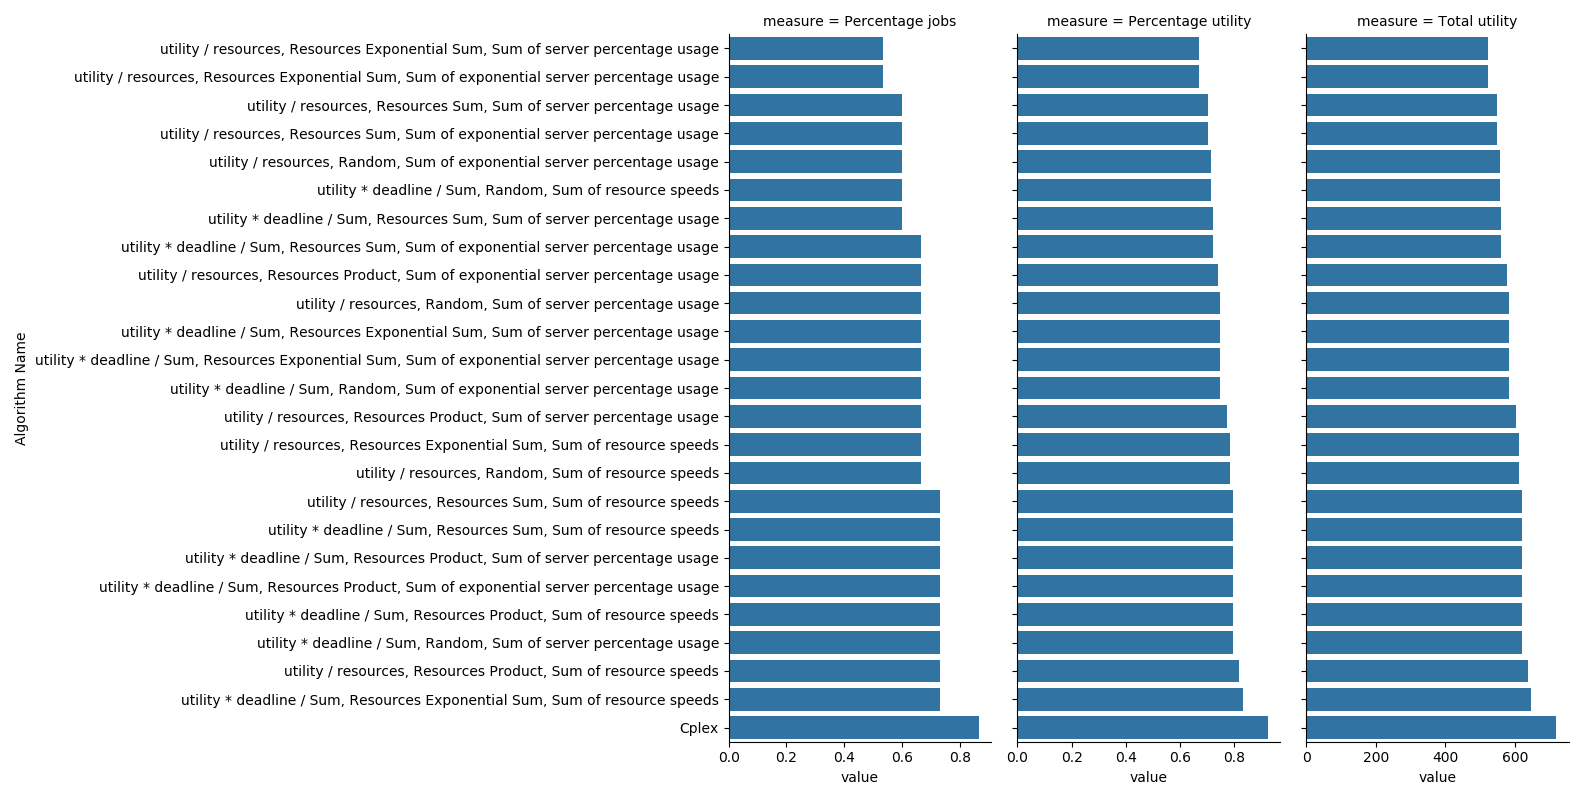
\includegraphics[width=1\linewidth]{../results/repeat_algorithms.png}
    \caption{Algorithm Results}
\end{figure}

\begin{figure}
    \begin{subfigure}{0.5\textwidth}
        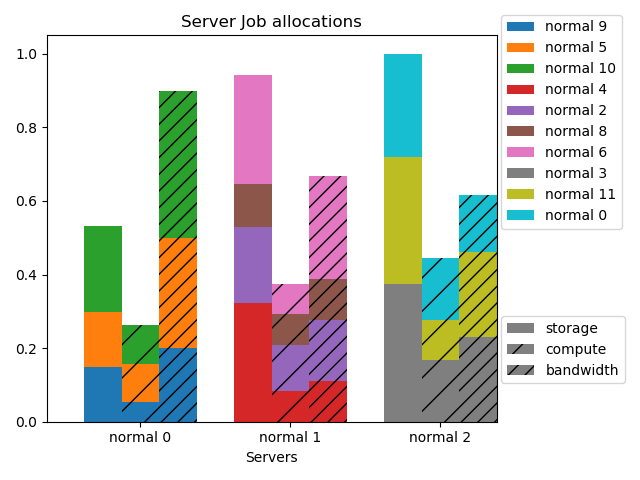
\includegraphics[width=1\linewidth, height=5cm]{../results/greedy_allocation.png}
        \caption{Example Greedy Allocation}
    \end{subfigure}
    \begin{subfigure}{0.5\textwidth}
        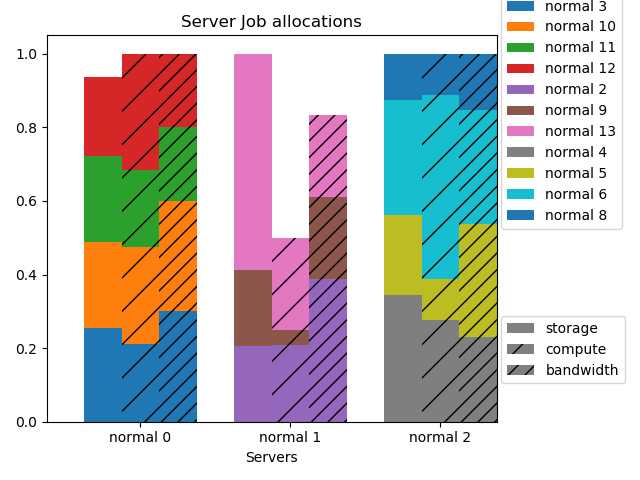
\includegraphics[width=1\linewidth, height=5cm]{../results/optimal_allocation.png}
        \caption{Example Optimal Allocation}
    \end{subfigure}
    \caption{Example jobs and servers}
\end{figure}

\section{Auction Idea}\label{sec:auction-idea}
The main idea was that currently most job work out how much resources that they require to run and so bid for that amount of required results however in doing this they are unaware of other jobs and their requirements. Therefore there is both a competition and cooperation involved we believe that can increase the total social welfare for everyone if people work together while in the mean time allowing the job to not give away its utility as in VCG auctions.
In real life then server will want to payed to the work that it does however to do this is not easy as the server allocate the resource price dynamically and as a job may not want to reveal its utility.
We have created an iterative VCG auction.

\subsection{Auction algorithm}\label{subsec:auction-algorithm}
\begin{lstlisting}[language=Python]
unallocated_jobs = jobs.copy()
while len(unallocated_jobs):
    job = choice(unallocated_jobs)

    # Calculate the minimum job price on all of the servers
    job_price, allocation_info = min((evaluate_job_price(job, server, epsilon=epsilon)
                                     for server in servers), key=lambda bid: bid[0])

        if job_price <= job.utility:
            # Uses the allocation info to create the new allocation on the selected server
            allocate_job(job_price, job, allocation_info, unallocated_jobs)
        else:
            # Remove job as there are minimum server is greater than the job's utility
            unallocated_jobs.remove(job)
\end{lstlisting}
\section{Auction Results}\label{sec:auction-results}
\begin{figure}
    \begin{subfigure}{0.5\textwidth}
        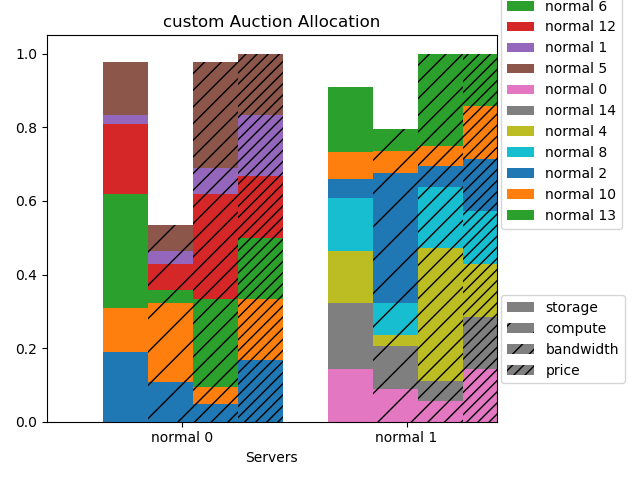
\includegraphics[width=1\linewidth, height=5cm]{../results/vcg_auction.png}
        \caption{Example VCG Allocation}
    \end{subfigure}
    \begin{subfigure}{0.5\textwidth}
        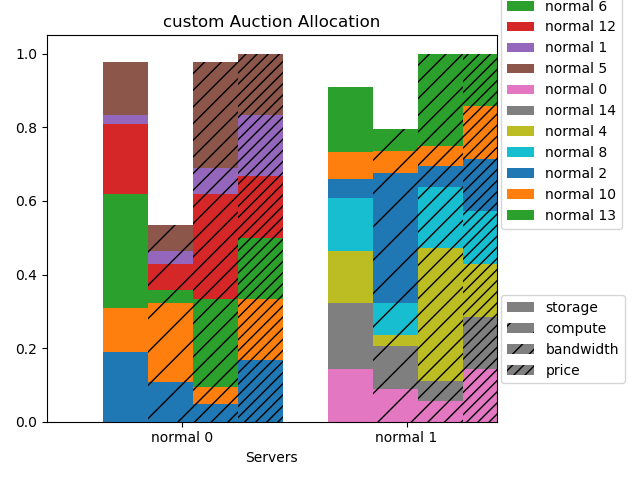
\includegraphics[width=1\linewidth, height=5cm]{../results/custom_auction.png}
        \caption{Example Custom Allocation}
    \end{subfigure}
    \caption{Example of auction results}
\end{figure}

\end{document}
